\documentclass[10pt]{article}

% Math formatting
\usepackage{amsmath}
\usepackage{amssymb}

\usepackage{subfigure}

% Lay out packages
\usepackage[margin=3cm]{geometry}
\usepackage[utf8]{inputenc}
%\usepackage{mathpazo}

% Dutch style of paragraph formatting, i.e. no indents. 
\setlength{\parskip}{1.3ex plus 0.2ex minus 0.2ex}
\setlength{\parindent}{0pt}

% Command for Horizontal lines
\newcommand{\HRule}{\rule{\linewidth}{0.5mm}}
% Command for degree symbol
\newcommand{\degree}{\ensuremath{^\circ}}

% Add images and pdf pages
\usepackage{graphicx}
\usepackage{pdfpages}

% Colored rows in tables
\usepackage[table]{xcolor}

% Clickable links with hyperref package
\usepackage[pdfborder={0 0 0 0}, linkcolor=black, urlcolor=blue]{hyperref}

% Fancy Header
\usepackage{fancyhdr}
\pagestyle{fancy}

% Psuedo code
\usepackage{algorithm}
\usepackage{algorithmic}

\rhead{\large\bfseries Assignment 2} % right header: document title
\lhead{\textsc{Jurriaans}, \textsc{Latour} \& \textsc{van der Molen}} % left header: document author
\cfoot{\large \thepage} % center footer: page number

\setlength{\headheight}{18pt}

\begin{document}

\begin{titlepage}
\begin{center}

\includegraphics[width=1\textwidth]{img/uva}\\[1cm]
\HRule \\[0.4cm]
% Title
 Assignment 2\\\small (Multi-Agent) Reinforcement Learning\\[0.4cm]
\HRule \\[1cm]
\begin{tabular*}{0.95\textwidth}{@{\extracolsep{\fill}} l c r}
Robrecht \textsc{Jurriaans} & Sander \textsc{Latour} & Hessel \textsc{van der Molen}\\
\textsc{5887380} & \textsc{5743044} & \textsc{5619785}\\
\end{tabular*}
\\[0.4cm]



\vfill \today
\end{center}
\end{titlepage}

% \newpage
% \thispagestyle{empty}
% \mbox{}
% \pagebreak

% \setcounter{tocdepth}{2}
% \tableofcontents
% \pagebreak


\section{Introduction}\label{introduction}
%\input{introduction}
% use reinforcement learning
In this paper it is shown how reinforcement learning can be used to solve the problem of capturing prey with multiple predators in the pursuit-domain\footnote{http://www.cs.cmu.edu/afs/cs/usr/pstone/public/papers/97MAS-survey/node8.html}. In this domain, multiple predators need to capture one or more prey in a toroidal world. This is done by, instead of describing a strategy based on rules, letting the predators learn the optimal actions by means of reinforcement learning. This paper describes two sets of experiments that were run on a configuration with two predators and one prey. In the first set of experiments both predators learn independently of each other. In these experiments a prey is captured when both predators surround the prey. In the second set of experiments the predators learn cooperatively, without communication, to capture the prey. In these experiments a prey is captured when at first both predators surround it and in the next move only one predator attacks the cell of the prey.

\paragraph{Overview of Paper}
In section \ref{theory} we will describe how reinforcement learning works and in section \ref{application} we will describe how we can apply this to the pursuit-domain. In section \ref{experiments} we will describe the experiments we ran and what results we got. In section \ref{conclusion} we will draw a conclusion based on the results.


\section{Theory}\label{theory}
% Reinforcement learning, Q-learning
Reinforcement learning is a method of learning which is not completely supervised since there is no predefined optimal action for each state but also not completely unsupervised since we do have a prior idea of what actions are better than others. The way we can learn is by giving rewards for achieving certain goals and propagating these rewards back in time so that the agent learns to achieve these goals. If we are able to describe the full transition model we can simply use value-iteration in which we iterate over the entire state-space and propagate the rewards in states to the adjacent states and so find optimal actions in all states. This method is not applicable if we do not have the transition model and to overcome this we can sample from the state space. If we sample from the state space the problem becomes Q-learning in which we find the optimal Q*. The agent repeatedly interacts with the environment and observes the reward it gets and uses this to update its Q-values.

There are multiple methods we can use to implement Q-learning. One such method is to first have the agent start in a given state and let it interact with the environment until it finds a goal state. We can then update each of the states it has visited and update their Q-values accordingly. Such methods are Monte-Carlo methods. Monte-Carlo methods can be quite slow since the original episode can take quite a while since no learning is done while it is in an episode. To overcome this we can implement a method in which the agent travels from a state $s$ with and action $a$ to a new state $s'$ with a reward $r$ given to the action $a'$ it will take in $s'$. This method is known as SARSA. The update rule of SARSA is seen in equation \ref{eq_SARSA}.

\begin{equation}\label{eq_SARSA}
	Q(s_t,a_t) \leftarrow Q(s_t,a_t) + \alpha[r_{t+1} + \gamma Q(s_{t+1},a_{t+1})-Q(s_t,a_t)
\end{equation}

This update is done after every transition to a non-terminal state. If $s'$ is a terminal state than $Q(s_{t+1},a_{t+1})$ is defined as zero. SARSA is an on-policy method, because the agent follows the policy it is learning.

% Exploration
The problem with such methods is that is very well possible that the solution the agent finds is not optimal but instead a local minimum of Q. Q only converges to Q* if all state action pairs are visited an infinite amount of times. A method to implement this is to have the agent explore by selecting a random action with a certain probability. The problem with this is that the agent will not learn the optimal policy but instead a policy in which it keeps taking random actions. In practise we can lower the probability of a random action after a sufficient amount of episodes. A good method is to select a random action based on a Boltzmann distribution seen in equation \ref{eq_boltz} in which the agent takes the random action $a$ with probability $p(a|s)$.

\begin{equation}\label{eq_boltz}
	p(a|s) = \frac{exp(Q(s,a)/\tau}{\sum_{a'}\exp(Q(s,a')/\tau)}
\end{equation}



\section{Application}\label{application}
In the pursuit-domain the agents are the predators and the states are simply the current observation of the predator. The possible actions are the actions in which the agent either does not move or moves to an adjacent cell. Each step that does not lead to a terminal state has an associated reward of $-1$ so that the agent learns the optimal path as being the future reward that minimises the amount of steps. In the first case the predators both separately learn their own Q without taking into account that the other predator is also learning. Since the predators do not know what action the prey takes the transition model is unknown and it is necessary to use Q-learning. Although this will probably work very well for the simple capture method, the second capture method requires coordinated cooperation between the predators. For this we treat the two predators as one agent performing a joint action. This way each predator learns the other predators Q matrix as well so that it knows which action the other predator should take.

% Increase size of state space gradually
\subsection{State Space}
Since the state space is very large it is necessary to decrease the size of the state space. A simple method is to use a rough method to get close to the prey and then start learning. One could even stop learning with a negative reward every time the predator gets too far from the prey so that it only learns when it is close by. Another method is to simply give a strong negative reward when the predator is too far from the prey so that it learns to keep close to the prey. These methods can be improved by slowly expanding the state space until it is as large as the full state space so that it first learns around the prey and then expands it so that it learns in the full state space. The starting size of the state space is set to 7 cells Manhattan distance of the prey which results in a circle\footnote{circle in a world consisting out of squares} around the prey in which the predators can learn the optimal strategy.

Another method is to use the symmetry of the state space. For each state there are 7 other states which are basically the same state. These are the four mirrored states, one over x, one over y and one over x and y and the four rotations around the centre. It is possible to rotate and mirror the state so that the agent is always in the same quadrant and update all 8 states at once. This greatly decreases the size of the state space.

A final method is to use both predators at once. Both predators are in a defined state which is observed by each of the predators. Once the other predator takes an action we can update that state too within our own Q matrix since we observe the state $s$, the action $a$, the next state $s'$ and its action $a'$ and the reward $r$.


\section{Experiments}\label{experiments}
\subsection{Q-learning for independent agents}
When letting two predators both independently learn we found that after training for 50000 episodes that the average capture time without exploring was $18.8170$, averaged over 1000 episodes. In figure \ref{sarsa1} we can see the learning curve over 100000 episodes in which the exploration rate slowly decreases by letting $\epsilon$ degrade over time.

\begin{figure}[h!tb]
\centering
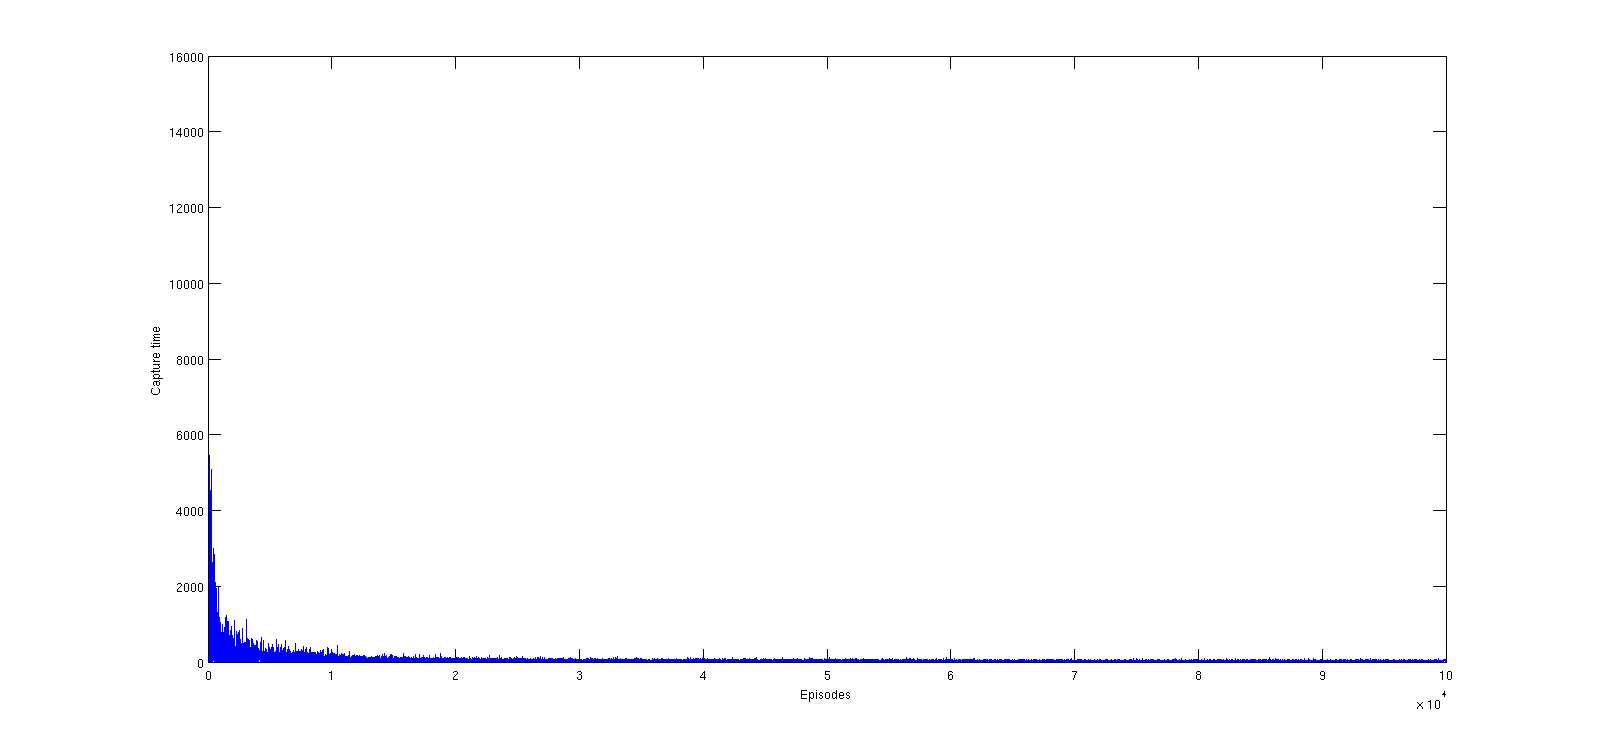
\includegraphics[width=0.9\textwidth]{img/sarsa1_explo_noexpan}
\caption{100000 episodes with decreasing $\epsilon$}
\label{sarsa1}
\end{figure}

If we bin the episodes in bins containing 1000 episodes we can see the effect more clearly as seen in figure \ref{sarsa1bins}. We see that after approximately 20000 episodes the capture times do not really improve. 

\begin{figure}[h!tb]
\centering
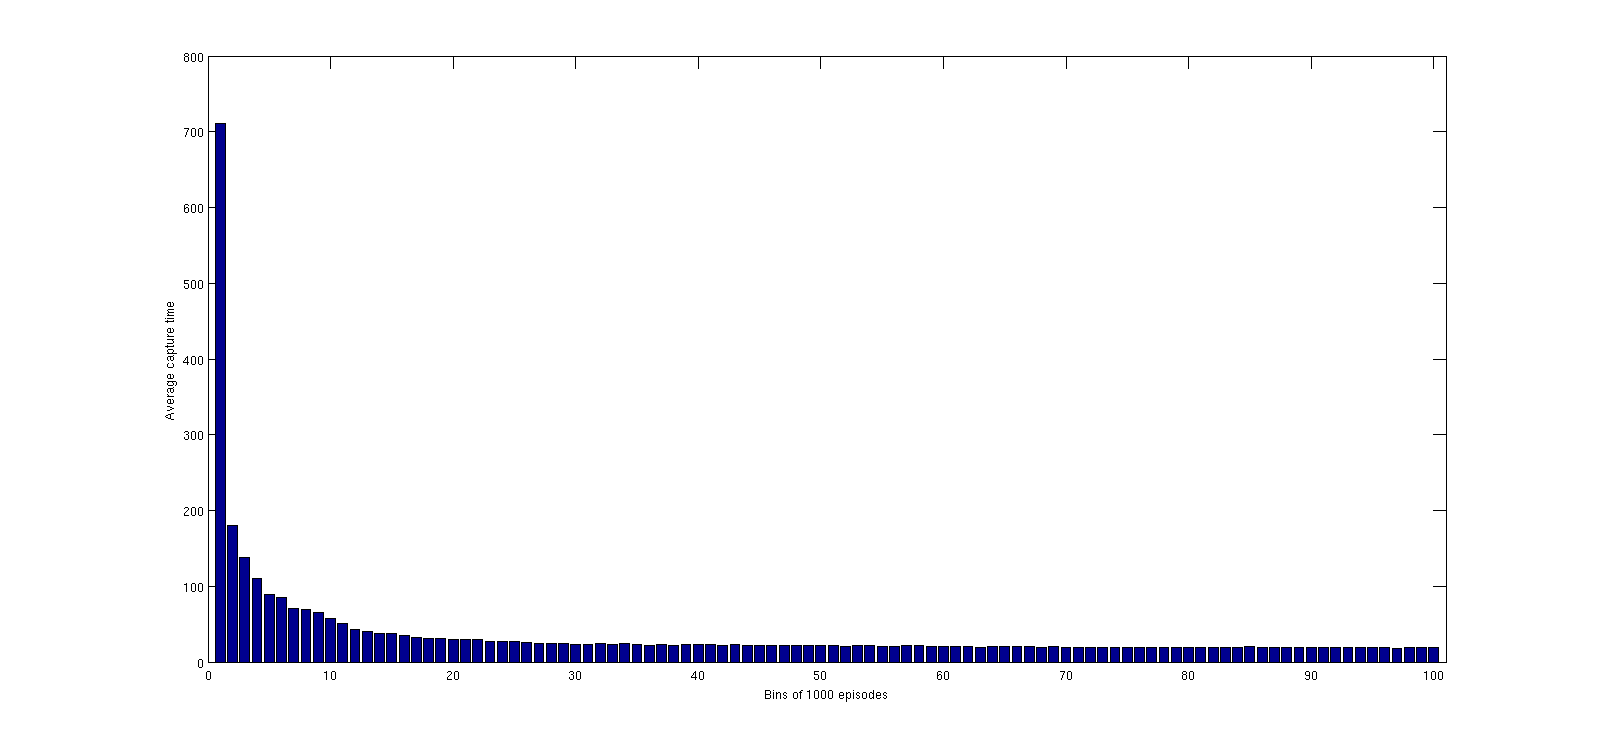
\includegraphics[width=0.9\textwidth]{img/sarsa_explor}
\caption{100000 episodes in bins of 1000 episodes}
\label{sarsa1bins}
\end{figure}

If we expand the state space by increasing the range in which Q-learning takes place every 1000 episodes we get the curve seen in figure \ref{expan}. We see that at some point the capture times start increasing again. This is due to the state space being expanded in a linear fashion, namely every 1000 episodes, while the state space it self increases exponentially because it is 2-dimensional.

\begin{figure}[h!tb]
\centering
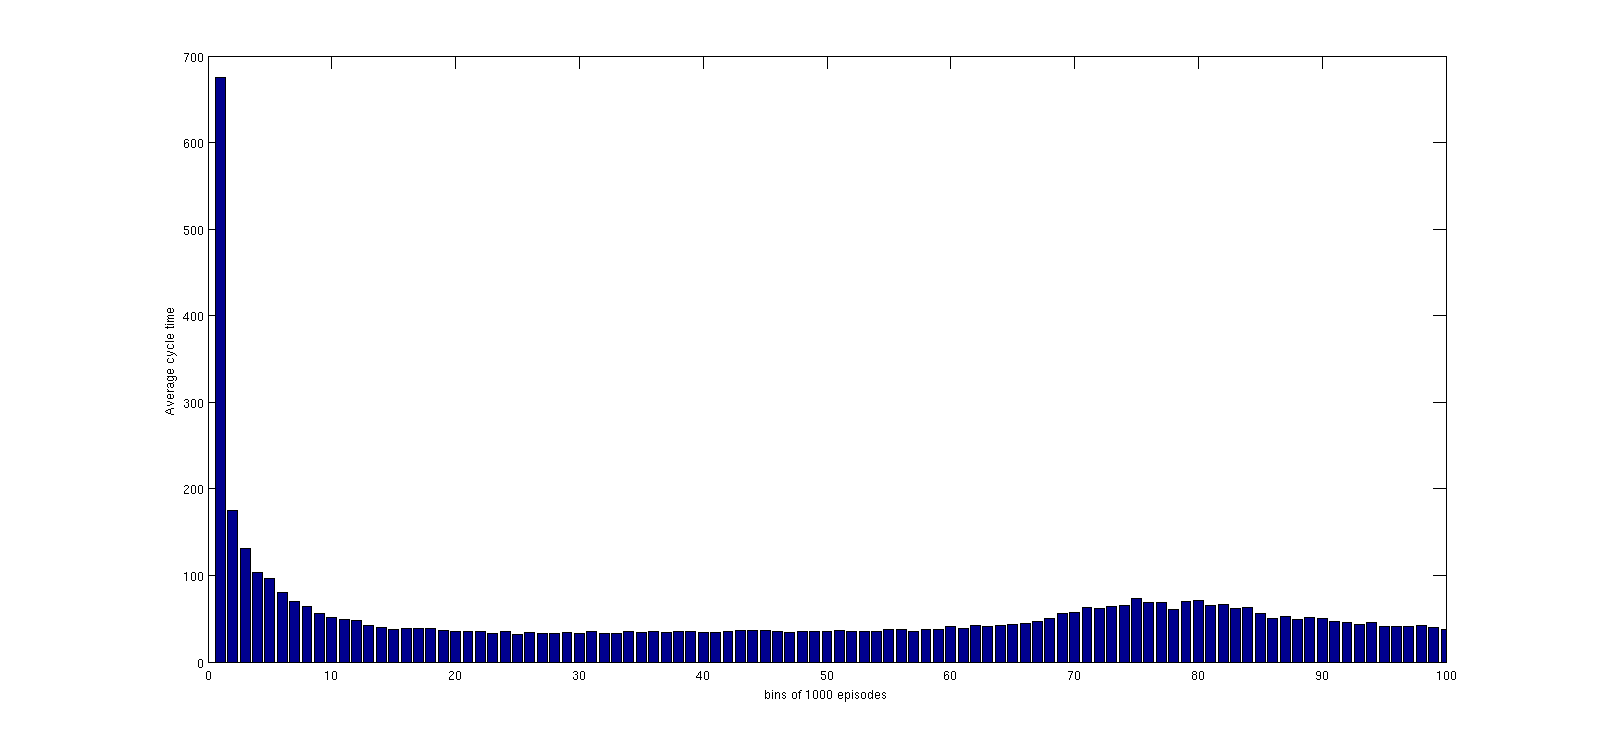
\includegraphics[width=0.9\textwidth]{img/expansion}
\caption{100000 episodes with an expanding state space}
\label{expan}
\end{figure}

When we change the capture method to the capture method which requires attacking the cell where the prey is located after first surrounding it with 2 predators we find that after training for 9000 episodes that the average capture time is $47.9$. As can be seen in figure \ref{cap4} learning starts fairly slow since the capture method is more complex than before.

\begin{figure}[h!tb]
\centering
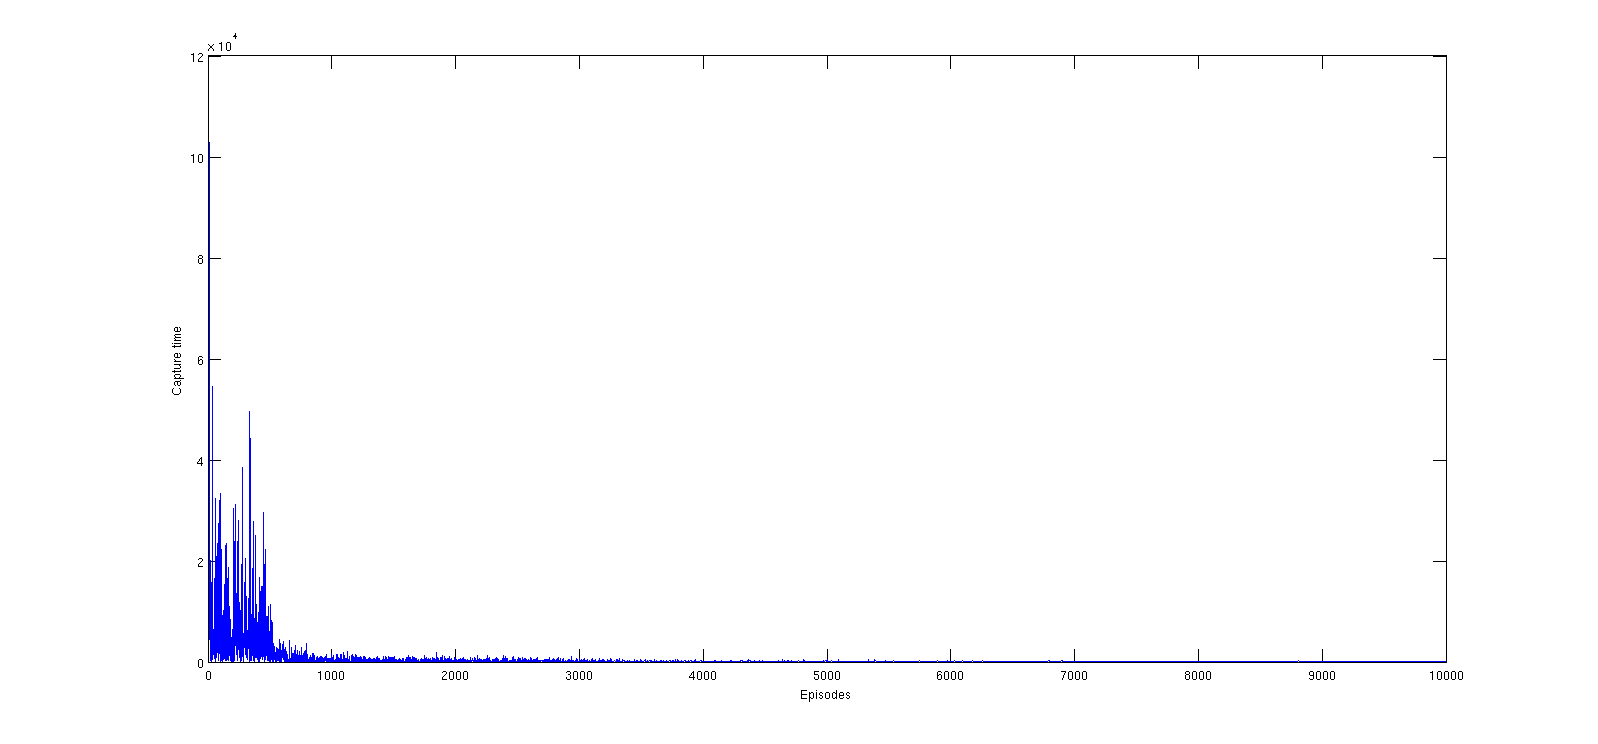
\includegraphics[width=0.9\textwidth]{img/cap4_ind}
\caption{10000 episodes with a more complex capture method}
\label{cap4}
\end{figure}

\subsection{Q-learning for cooperative agents}



\section{Conclusion}\label{conclusion}





% % References
%  \pagebreak
% 
%  \bibliographystyle{plain} % plain, nature, jbact
%  \bibliography{myref} 
%  
%  \pagebreak
%  \appendix
%  %\input{appendix}

\end{document}
